\documentclass{article}
\usepackage[utf8]{inputenc}
\usepackage[numbers,sort&compress]{natbib}
\usepackage{hyperref}
\usepackage{todonotes}
\usepackage{graphicx}
\usepackage{subfig}
\usepackage{amsmath}
\usepackage[toc,page]{appendix}
\usepackage{amssymb}
%\usepackage{gensymb}
\usepackage{soul}
\usepackage{placeins}

\title{Direct detection of dark matter}
\author{Peter Bosch, Max Briel and Jelle van Urk}
\date{June 2018}

\graphicspath{ {Images/} }

\begin{document}

\maketitle
\newpage
\tableofcontents
\newpage
Recommended article for programming:

https://arxiv.org/pdf/1002.1912.pdf

Review article about whole DM searches (including direct detection): \cite{Roszkowski:2017nbc}.

More theoretical: \cite{Queiroz:2017kxt}.

Probing WIMP particle physics and astrophysics with direct detection and neutrino telescope data:
https://arxiv.org/pdf/1410.8051.pdf

\section{Introduction}


- Observational clues for the presence of Dark Matter (Go more into this) 
Deviations from the galactic rotation curves and other astrophysical observations provide evidence for the presence of additional unobserved matter: Dark Matter. From the Cosmic Microwave background it has been deduced that this matter cannot be of baryonic nature and accounts for 63\% of the matter in the universe [REFERENCE], while only interacting gravitationally with ordinary matter. 
This lead to the idea of the WIMP particle, a Weakly Interacting Massive Particle, as an source of observed gravitational interactions. 
However, since its only weakly interacting with ordinary matter, its detection is a difficult task. This can either be achieved using a indirect detection, where products that can only come from Dark Matter interactions are observed. However, the possibility remains for other processes to give the same results. 

More concrete evidence can be provided by direct detection of dark matter interacting with standard model matter. A Weakly Interacting Massive Particle is expected to have these interactions through the weak force. Direct detection experiments focus on measuring a recoil effect from collisions of dark matter particles with ordinary matter.

\FloatBarrier
\section{Interaction Rate \small{\textit{Max Briel}}}

For direct detection experiments to draw conclusions from their measurements, it is important to know the expected rate of WIMP interactions in the detector. Because a WIMP can scatter elastically and inelastically of matter, this section will consider the general components of the interaction rate, while specific properties will be discussed in the corresponding sections. \todo{Add reference to the right section}

A simple first approximation of the interaction rate would be an exponentially decay with recoil energy ($E_R$) with dependencies on the WIMP mass ($m_\chi$) and detector particle mass ($m_T$). 

\begin{equation}
    \frac{dR}{dE_R} = \frac{R_0}{E_0 r} e^{-E_R/E_0r}, \quad \mbox{with } r = \frac{4m_{\chi} \cdot m_T}{(m_{\chi} + m_T)^2}, 
\end{equation}
where $E_0$ the most probable dark matter kinetic energy, and $R_0$ the total event rate \cite{Lewin:1995rx}. This is a extremely crude approximation for the expected number of events, which neglects important details in the interaction rate curve. Lewin and Smith provide an overview of corrections to the rate \cite{Lewin:1995rx}. 

First of all, the movement of the Earth and Sun through the Galaxy alter the rate at which the dark matter particles go through the Earth \cite{Spergel:1987kx}. Assuming a stationary dark matter distribution in our Galaxy, the dark matter flux increases when the Earth moves into the same direction as the Sun and vice versa. This will be discussed further in section \ref{Local_DM_Density} and \ref{DM_Velocity}.

Secondly, properties of the detector alter the number of interactions that are expected. These range from more practical aspects, such as the resolution of the photomultipliers, to the type of material used in the detector. Moreover, the efficiency with which nuclear and electronic recoil events can be distinguished determines the accuracy of the measured rate at a recoil energy.

Furthermore, the WIMP interaction can be dependent on the spin. Spin-independent interactions provide a stronger signal due to its scalar nature and coherent nature at low energies. And finally, due to the particle wavelength being smaller than the radius of the target a correction to the cross section has to be applied, called the form factor.

\begin{equation} \label{interaction_rate}
    \frac{dR}{dE_R}(E,t) = \frac{\rho_0}{m_\chi \cdot m_T} \int_{v_\text{min}}^{v_\text{max}} v \cdot f(\textbf{v},t) \frac{d \sigma}{dE_R} (E, v)d^3v
\end{equation}

These corrections are combined to form a complete picture of the interaction rate per kg detector material (Eq. \ref{interaction_rate}) \cite{Lewin:1995rx, Undagoitia:2015gya}. $\rho_0$ is the local dark matter density, $f(\mathbf{v}, t)$ the velocity distribution of dark matter particles, and $\tfrac{d\sigma}{dE}$ its differential cross section through which the particle physics enters, such as the cross section and form factor, which can depend on the spin. $\sigma_0$ is the cross section at zero momentum and depends on the type and spin dependence of the interaction. \todo{mention the dark matter mass dependence in the interaction rate}

\begin{equation} \label{Eff_cross}
    \frac{d\sigma}{dE_R} = \frac{m_T}{2\mu_T^2 v^2} \left( \sigma_0^\text{SD} F^2_\text{SD}(E_R) + \sigma_0^\text{SI} F^2_\text{SI}(E_R)\right)^2
\end{equation}

\subsection{Form Factor \small{\textit{Max Briel}}} \todo{Maybe add a picture of the parametrisation?}

During the collision momentum is transferred between the particles. If this momentum exchange is extremely small, its wavelength can be smaller than the radius of the particle. This results in lost of coherence and a decrease in the effective cross section, which is implemented by the form factor. 
The spin-independent form factor is calculated using a Fourier transform of the scattering centres assuming they follow the same distribution as the charge density \cite{Lewin:1995rx}. Since this involves an integral that has to be numerically solved, it is more common to use the Helm form factor, which is an analytical approximation \cite{Helm:1956zz}.

\begin{equation} \label{Helm}
    F^2_\text{SI} = \left[ \frac{3 j_1(qR_1)}{qR_1} \right]^2 e^{-q^2 s^2}, 
\end{equation}
where $j_i$ is the spherical Bessel function of the first kind and $q = \sqrt{2m_T E_R}$ the momentum transfer. The other variables determine the parametrisation and come from spectroscopy experiments \cite{Fricke:1995zz}. Shell-model \cite{Vietze:2014vsa} and Hartree-Fock calculations \cite{Co:2012adt, Duda:2006uk} have shown that the Helm parametrisation deviates the total event rate less than 5\%. Furthermore, equation \ref{Helm} shows that the form factor suppresses the event rate at high recoil energies. This is more present with high mass target particles, because $\sigma_0$ has a quadratic dependence on its mass number, increasing the form factors effect \cite{Undagoitia:2015gya}.
\todo{Image of this effect?}

\begin{equation} \label{SD_Form}
    F^2_\text{SD} = \frac{S(E_R)}{S(0)}
\end{equation}

\begin{equation} \label{Response}
    S(E_R) = a^2_0 S_{00}(E_R) + a_0a_1S_{01}(E_R) + a_1^2 S_{11}(E_R)
\end{equation}

To determine the spin-dependent form factor, the type of scattering particle has to be determined. For an interaction with a nucleus the form factor can be rewritten as a normalised response function of an ensemble of spin-1/2 particles (Eq. \ref{SD_Form}) and consists of spin structure functions (Eq. \ref{Response}) \cite{Cannoni:2011iu}. These are often calculated using nuclear shell-models \cite{Ressell:1997kx,Toivanen:2009zza}, but other atomic models can lead to different spin structure functions \cite{Ellis:1987sh, Engel:1989ix, Iachello:1990ut}. Cerde$\tilde{\text{n}}$o et al.\cite{Cerdeno:2012ix} proposed a parametrisation that mimics the median value of a collection of spin structure calculations to solve this problem. 

\begin{equation}
    S_{ij} = N((1-\beta)e^{-\alpha u} + \beta), 
\end{equation}
where $\alpha$, N, and $\beta$ are parameters determined from measurements, while $u = (qb)^2/2$ consists of $q$,the momentum transfer and $b$ as shown in equation \ref{b}.
 \begin{equation} \label{b}
     b = \sqrt{\tfrac{41.467}{45.0A^{-1/3}-25.0A^{-2/3}}}
 \end{equation}

The WIMP particle could also scatter of an electron. Since the electron is in a bound state, two competing processes affect the effective cross section. This results in a more complex form factor consisting of a Sommerfeld enhancement \cite{ArkaniHamed:2008qn} and suppression from the need to overcome the binding energy \cite{Essig:2011nj}.\todo{Maybe write a little more about the electron form factor? Difference between atoms vs crystals?}

More details mathematics for the calculation of WIMP interactions have been proposed, such as non-relativistic Effective Field Theory \cite{Fitzpatrick:2012ib}. This could give a better description of the effective cross section of the collision and possibly make it impossible to compare direct detection experiments with different target material \cite{Schneck:2015eqa}. 

\subsection{Velocity Distribution \small{\textit{Jelle van Urk}}} \label{DM_Velocity}

\begin{itemize}
    \item annual modulation \cite{Undagoitia:2015gya} for more references
\end{itemize}

Velocity Distribution:
Maxwellian distributed, Earth moving through halo, vmin and vmax of elastic scattering. \cite{Kavanagh:2014rya} Why Maxwellian, shape of halo. 
Or non-Maxwellian, difference in shape distribution. 
As mentioned in section 2.1, the expected recoil rate is necessary 

\begin{equation}
    v_{min} = \sqrt{\frac{m_{N}E_{R}}{2\mu^{2}_{N}}}
\end{equation}

https://arxiv.org/pdf/1002.1912.pdf
\begin{figure}[h]
    \centering
    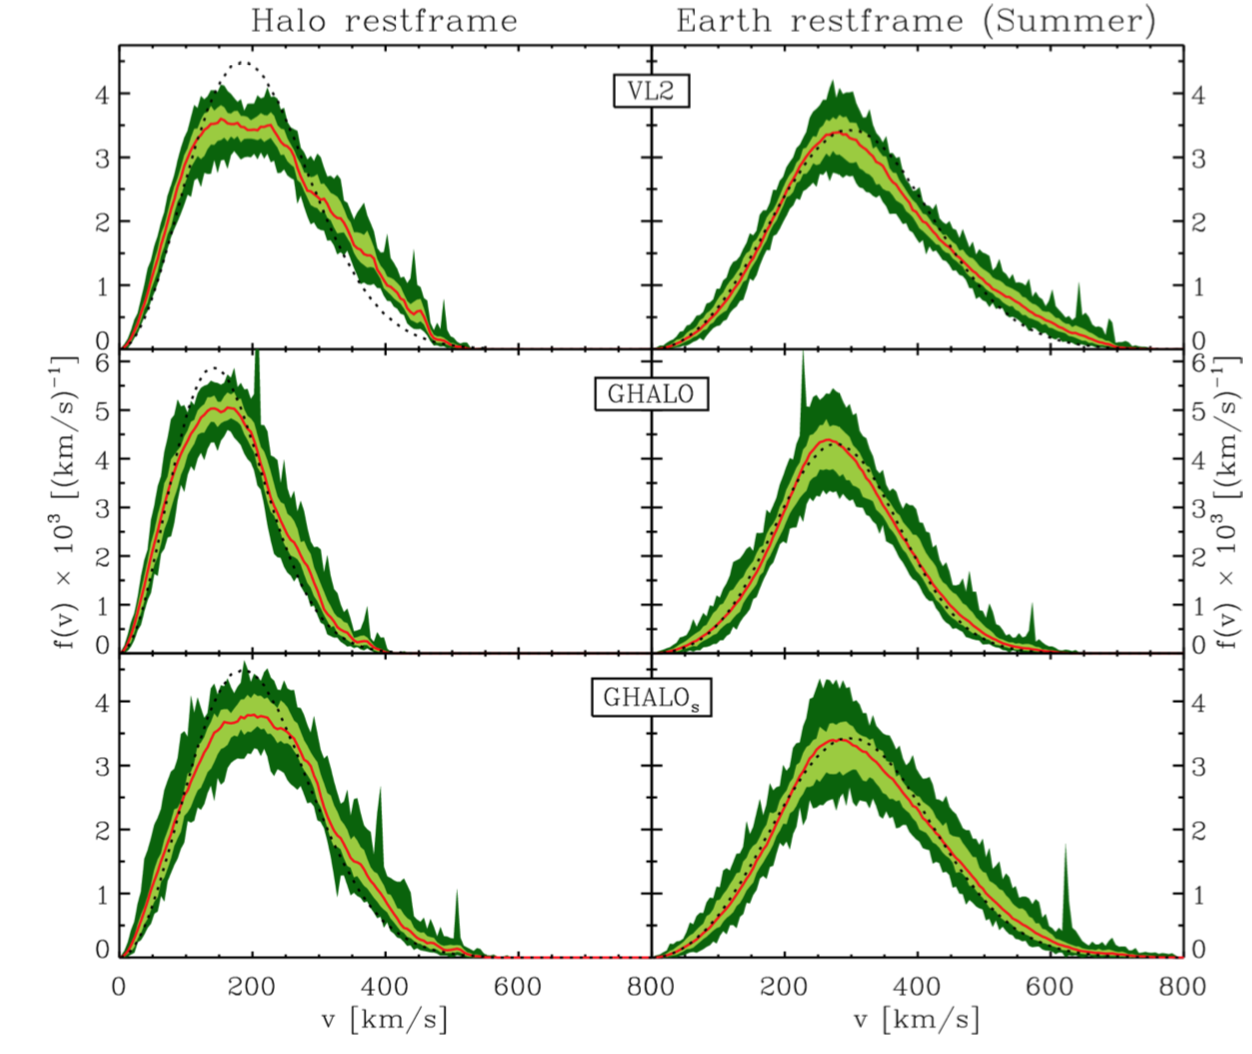
\includegraphics[width=0.7\textwidth]{Vel-dist.png}
    \caption{}
\end{figure}


\begin{equation}
    f(\textbf{v}) = \frac{1}{\sqrt{2\pi}\sigma}e^{-\frac{|\textbf{v}^{2}|}{2\sigma^{2}}}
\end{equation}

\section{Local Dark Matter Density \small{\textit{Jelle van Urk}}} \label{Local_DM_Density}

%What is the local distribution of dark matter and what are its properties?
%https://arxiv.org/abs/1404.1938
%Local dark matter density:
%The local dark matter density, H1 and 2, 
%Method 1: Jeans equation, z-direction. Movement of stars of neighbourhood of Sun.  
%Method 2: Spherical shell and local dark matter. 
To get a better insight in the scattering interaction rate it's important to have some measurements in the local dark matter density ($\rho_{DM}$), because $\frac{dR}{dE_{R}}$ is directly proportional to this density. The local DM density gives the density in close neighbourhood of the SUN, usually around 100 - 1000pc. Older measurements give an local density of $0.542 \pm 0.042 \frac{GeV}{cm^{3}}$ (ref) and $0.25 \pm 0.09 \frac{GeV}{cm^{3}}$ (ref). Clearly they're not even similar within their uncertainties. Mainly because both used different data sets and assumptions in their methods. Therefore new calculations are done with the least amount of assumptions. In the next sections we will describe two of methods. The first uses the vertical motion of nearby stars, also called 'tracers' (ref). These motions are described with Jeans equations. The second is a global measure, which uses the rotation curve of the Milky Way to extrapolate the local DM density. \\
In figure ... a history of local DM density measurements is shown over the last century. The first measurement was done by Kapteyn in 1922, who was the first who claimed to have proved the existence of dark matter. However, in the following decades his method was corrected and extended. In the late 80's there was a boost in the measurements, since new satellites were able to look at around 100.000 stars in a 100 pc radius. The different colors in the circles point out a different method used the determine the density: the values in blue are calculated from a surface density, the red one used the rotation curve and the green circle used a different assumption the surface density (ref). The grey band is $\rho_{DM,ext}$, the extrapolation of the rotation curve. 
\FloatBarrier
\begin{figure}[h!]
    \centering
    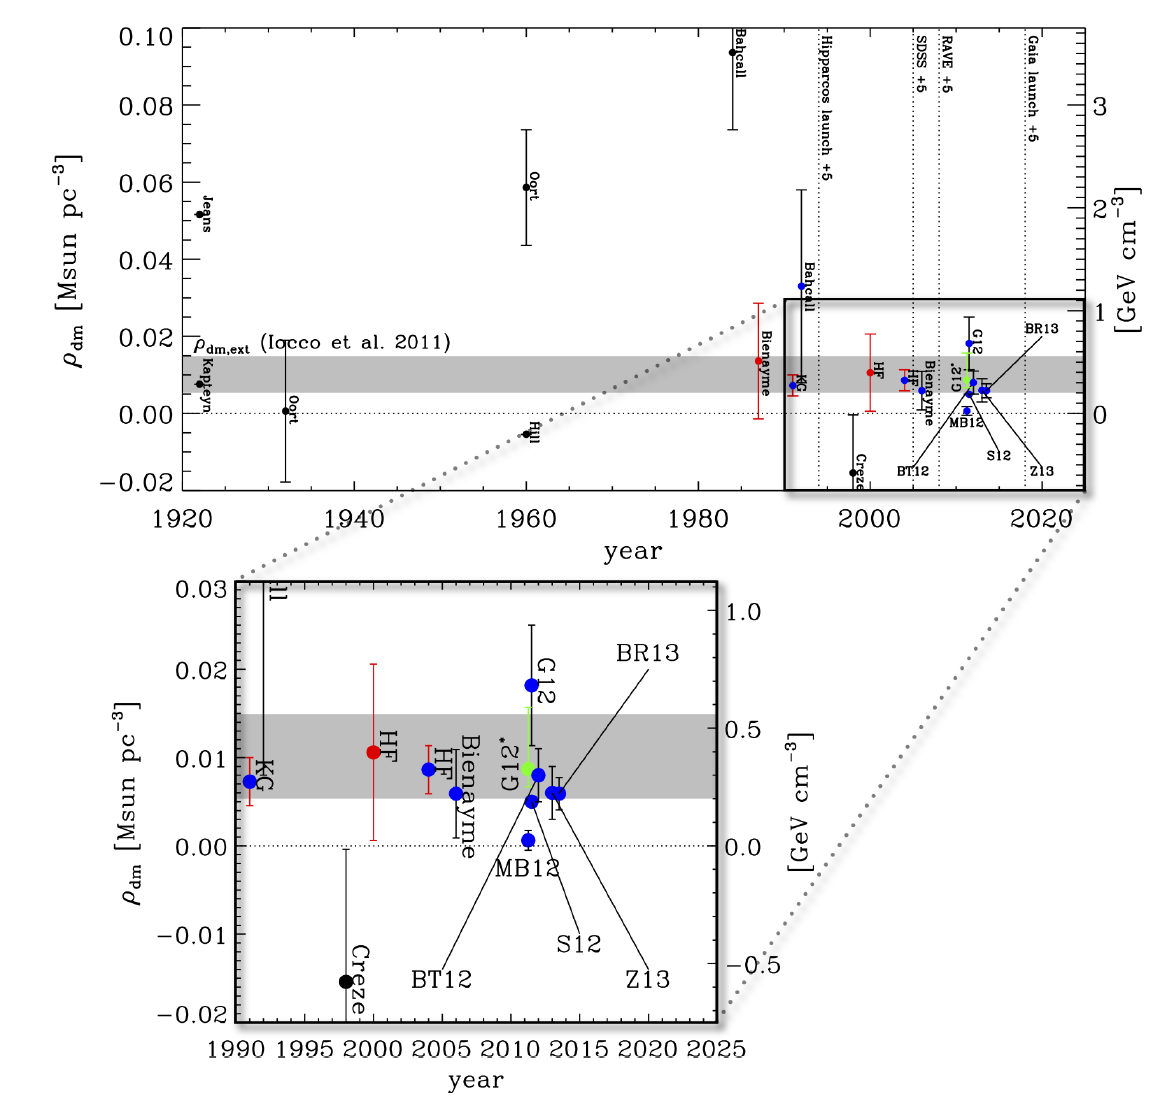
\includegraphics[width=\textwidth]{Century.png}
    \caption{}
\end{figure}


\begin{figure}[h]
    \centering
    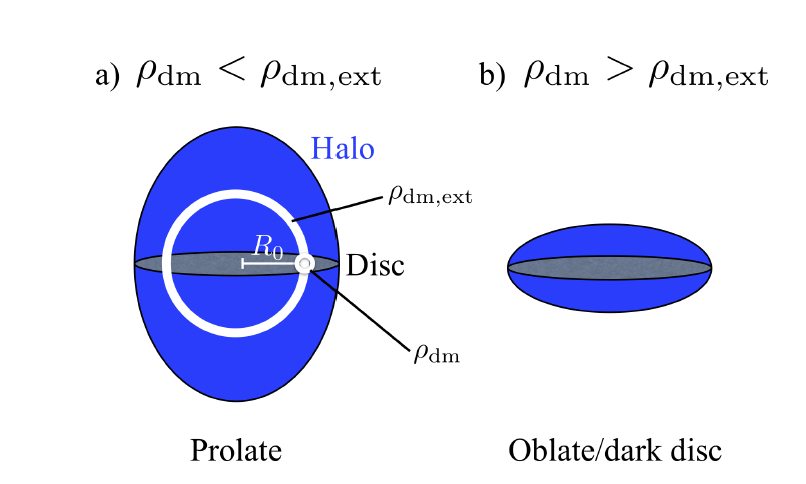
\includegraphics[width=0.7\textwidth]{Halo.png}
    \caption{}
\end{figure}

\subsection{Extrapolation of $\rho_\text{DM}$}

\subsection{Tracer stars model}
The first method uses the vertical movement of neighbouring stars, also known as 'tracer stars'. In this system the stars obey the collisionless Boltzmann equation:
\begin{equation}
    \frac{df}{dt} = \frac{df}{dt} + \nabla_{x}f\cdot \textbf{v} - \nabla_{v}f\cdot\nabla_{x}\Phi = 0,
\end{equation}
where f is the distribution function of the surrounding stars. \textbf{v} and \textbf{x} are the velocity and position. The remaining $\Phi$ corresponds to the gravitational potential. If the system was in dynamical equilibrium, which isn't the case, we could directly calculate the gravitational forces between the stars. For out purposes we need to integrate this equation, which results in the Jeans equations (ref). We are interested in the z-direction of the stars, so we take the vertical component of these equation:

\begin{equation}
    \frac{1}{R\nu}\frac{\partial}{\partial R}(R\nu \sigma_{Rz}) + \frac{1}{R\nu}\frac{\partial}{\partial \phi}(\nu \sigma_{\phi z}) + \frac{1}{\nu}\frac{d}{dz}(\nu \sigma_{z}^{2}) = -\frac{d\Phi}{dz},
\end{equation}

where the first term is the 'tilt' term (T). This term couples the vertical and radial motion of the tracers. The second term is the 'axial' term (A), which does the same for the vertical and axial motions. The right hand side of this equation is the vertical acceleration K. Integrating both sides with respect to $z$ gives us the necessary expression for $\sigma_{z}^{2}$, which is the vertical velocity dispersion:

\begin{equation}
    \sigma_{z}^{2}(z) = \frac{1}{\nu(z)}\int_0^z\nu(z')[K_{z}(z')-T(z')-A(z')]dz' + \frac{C}{\nu(z)}. 
\end{equation}





% General information about the interaction rate. 
% - General form
% - Form Factor
%   - which is due to the finite size of the nucleus and dependent principally on nuclear radius and recoil energy. This also differs for spin-dependent and spin-independent interactions.
%   - 

% - Velocity distribution
% - Dark matter density distribution
% 

\FloatBarrier
\section{Elastic Scattering \small{\textit{Max Briel}}}

The two main interaction mechanism between WIMPS and ordinary matter are elastic and inelastic scattering. The idea for elastic scattering of Dark Matter was introduced in 1984 by Goodman \& Witten \cite{Goodman:1984dc} and can produce a nuclear recoil effect necessary for measurement, while the momentum is conserved \cite{Undagoitia:2015gya, Lewin:1995rx}. This can take place in a spin-dependent and spin-independent fashion. 

\begin{figure}[h]
    \centering
    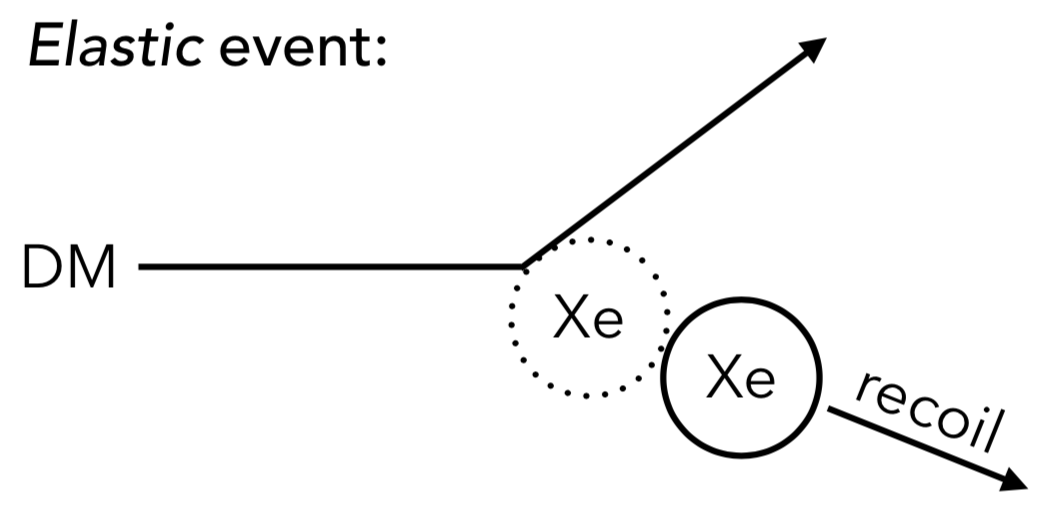
\includegraphics[width=0.7\textwidth]{Elastic_Scattering.png}
    \caption{Dark matter particle elastically scattering of a Xenon atom that recoils due to the collision. Image from \cite{McCabe:2015eia}.}
    \label{elastic}
\end{figure}


\subsection{Spin-independent \small{\textit{Max Briel}}} \todo{I want to write more, but not sure about what}

In a WIMP scenario it is expected that spin-independent interactions provide the largest contribution to the effective cross section. This becomes clear if the cross section at zero momentum from equation \ref{Eff_cross} is written out. 

\begin{equation}
    \sigma^\text{SI}_0 = \sigma_{p \chi} \frac{\mu_T^2}{\mu_p^2} \left[Z \cdot f^p + (A-Z) f^n \right]^2
\end{equation}
There is a contribution to the WIMP interaction from the protons and neutrons in the nucleus with an interaction cross section between the WIMP and a proton $\sigma_{p \chi}$. Although other theories exists \cite{Yaguna:2016bga}, it is assumed in most cases that the interaction strength from the protons and neutrons with the WIMP are equal ($f^n = f^p$). This results in a $A^2$ dependence, where $A$ is the atom mass number. This enhancement is of the order $\sim 10^4$ \cite{Vietze:2014vsa} and, therefore, heavy mass atoms are used as a target material in most direct detection experiments.
However, the heavier mass number also increases the influence of the form factor on the event rate, which can cause a significant drop in interactions, as shown in figure \ref{nucleus mass influence}. Thus, different detectors can be sensitive in different regions. The spin-independent part can also completely vanish depending on the assumed nature of the WIMP particle \cite{Lewin:1995rx}.


\begin{figure}[h]
    \centering
    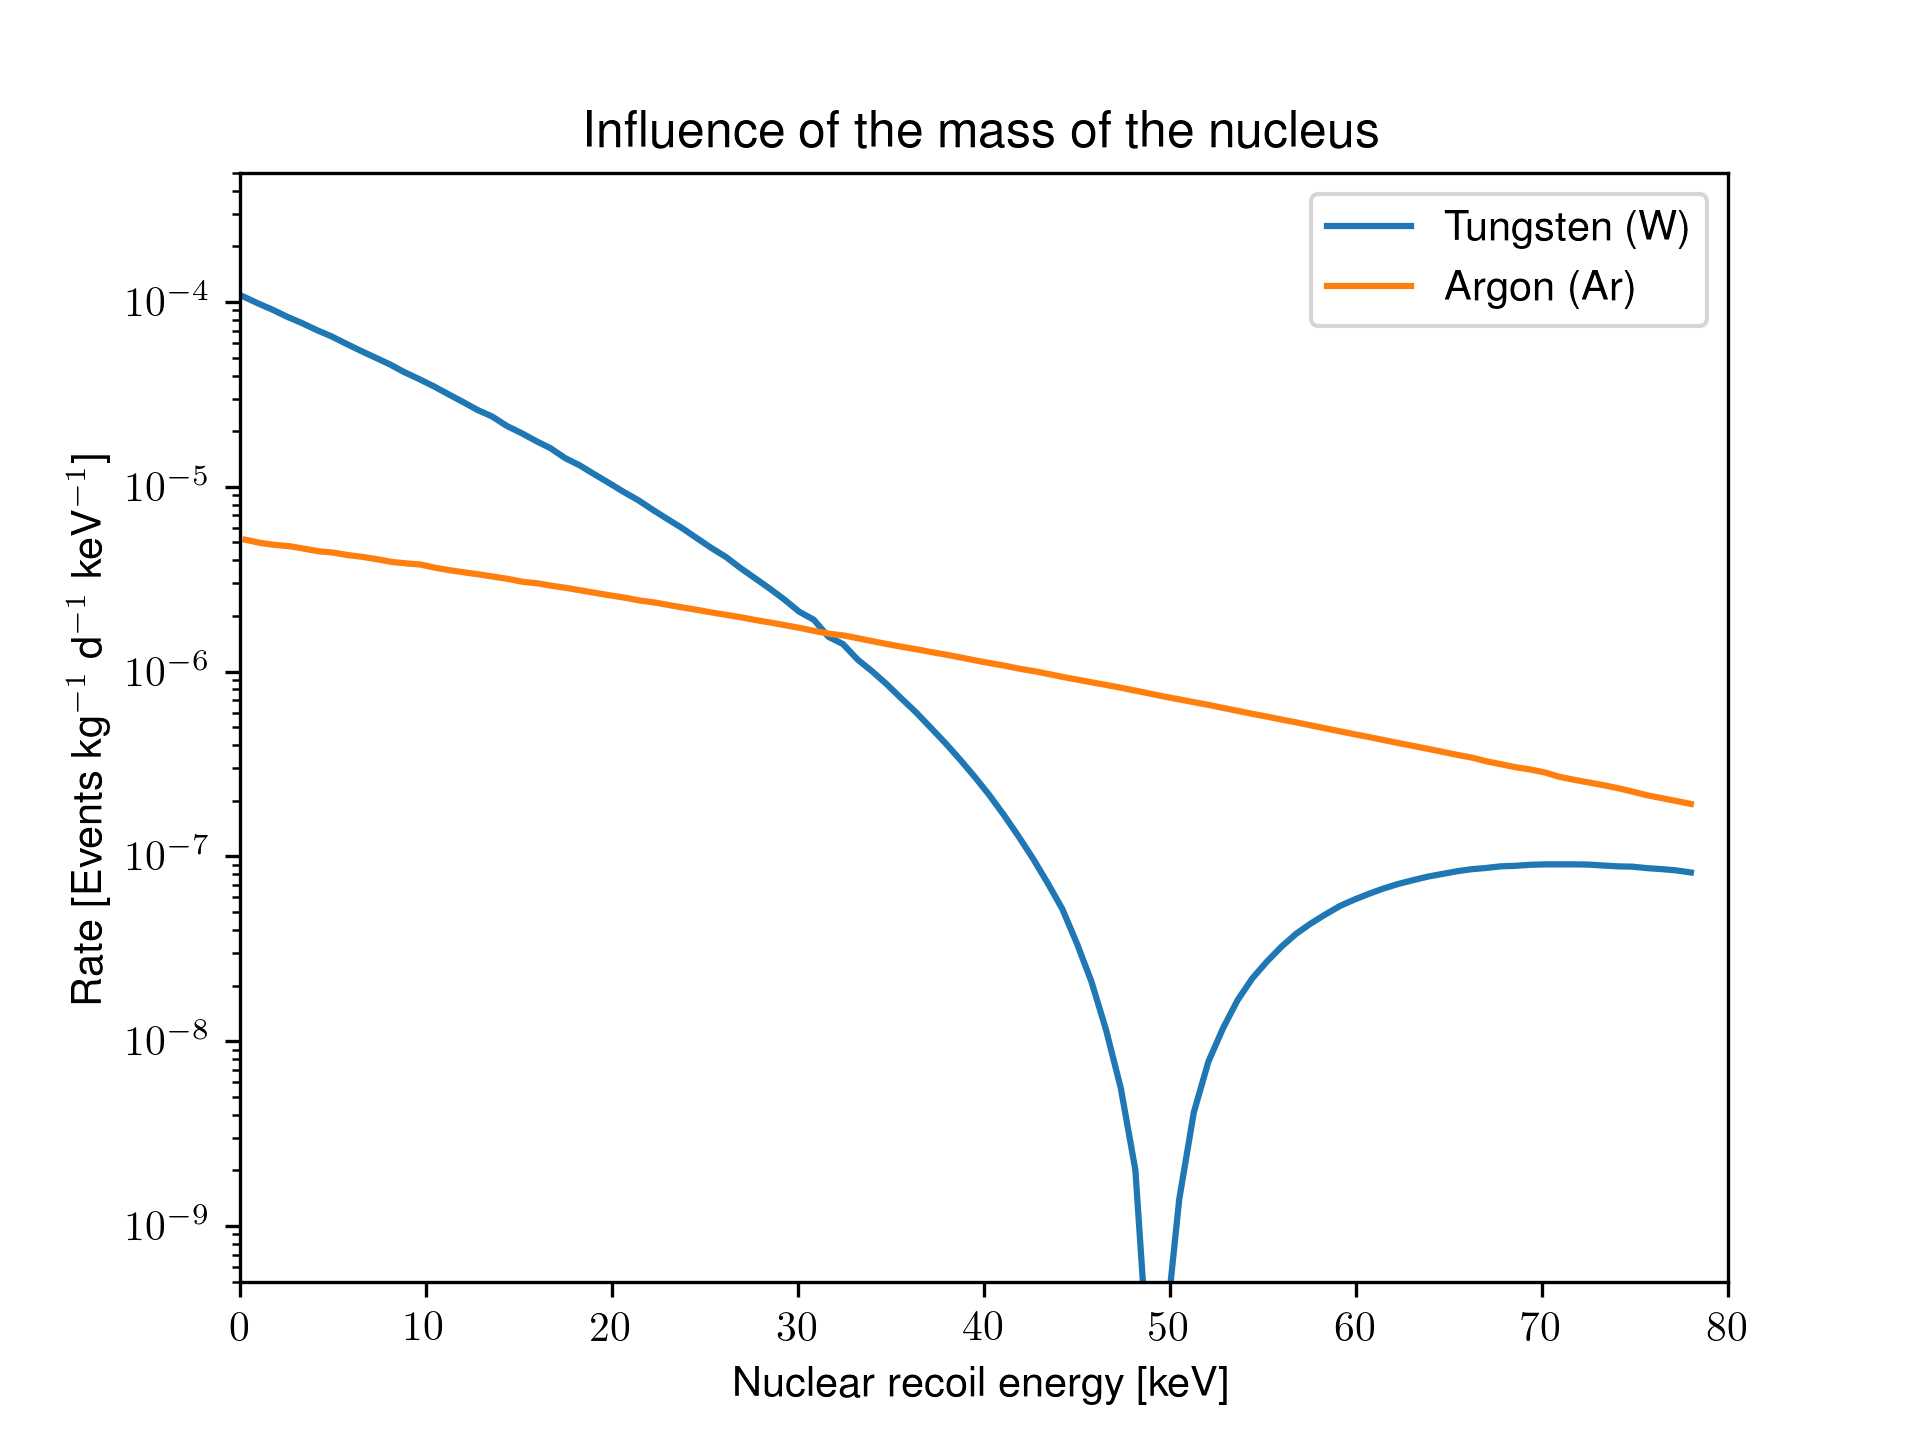
\includegraphics[width=0.7\textwidth]{mass_influence.png}
    \caption{The mass number of the target material alters the interaction rate by increasing the influence of the form factor. The data comes from \cite{Undagoitia:2015gya} with a WIMP mass of 100 GeV/$c^2$ and a cross section of $10^{-45}$ cm$^2$.}
    \label{nucleus mass influence}
\end{figure}


\subsection{Spin-dependent \small{\textit{Max Briel}}}

Since it is unknown if a dark matter particle can even spin-independently scatter of a nucleus, it is important to also look at possible spin-dependent interactions, even tough, the interaction strength is smaller. The corresponding zero momentum cross section is often expressed in average spin interaction $\langle S \rangle$ between the WIMP and neutrons \& protons. 

\begin{equation}
    \sigma^\text{SD}_0 = \frac{32}{\pi} \mu^2_T G^2_F \left[a_p \langle S^p \rangle + a_n \langle S^n \rangle \right]^2 \frac{J+1}{J}, 
\end{equation}
which depends on the total nuclear spin ($J$), Fermi coupling constant ($G_F^2$), and the effective coupling between the WIMP and nucleus particles ($a_p$ \& $a_n$) \cite{Undagoitia:2015gya}. The latter are often assumed to be the same \cite{Kavanagh:2014rya} and can be  calculated using chiral effective field theory currents \cite{Klos:2013rwa} or shell-model calculations \cite{Toivanen:2009zza}. 


\FloatBarrier
\newpage

\section{Inelastic Scattering \small{\textit{Max Briel}}} \todo{check if it doesn't state that inelastic scattering is always spin-dependent}

\begin{figure}[h]
    \centering
    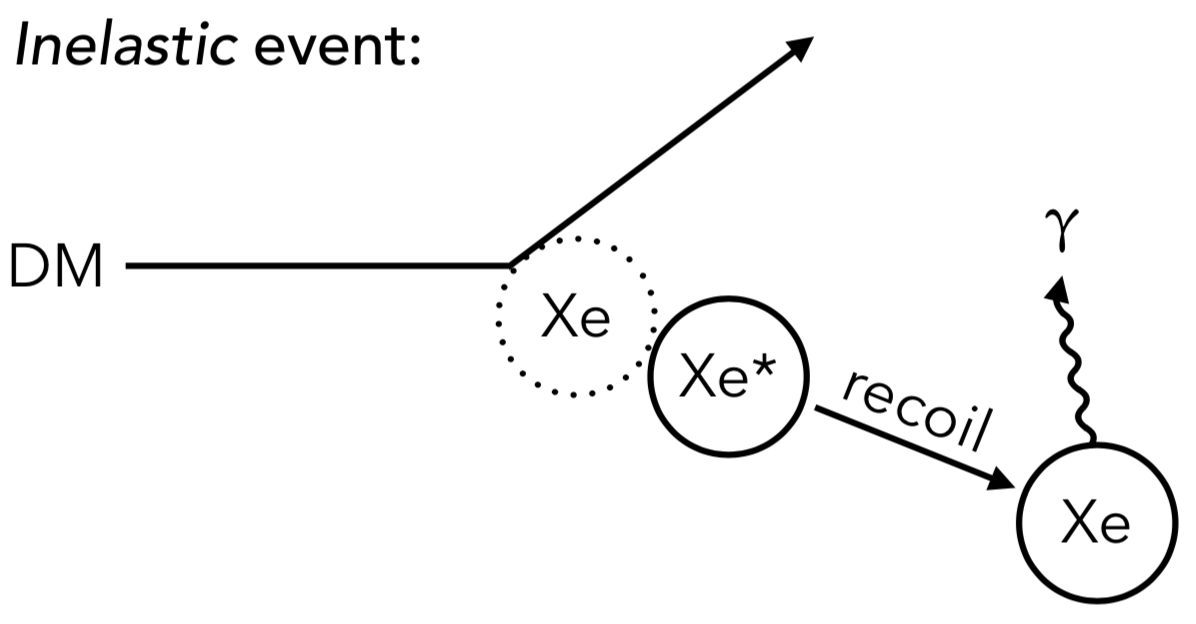
\includegraphics[width=0.7\textwidth]{Inelastic_Scattering.png}
    \caption{A dark matter particle scattering inelastically of a Xenon atom, which recoils and is put into an excited state. This is followed by a de-excitation and the emission of a photon. Image from \cite{McCabe:2015eia}.}
    \label{inelastic}
\end{figure}

Another possible interaction channel is inelastic scattering of the WIMP, during which one of the particles is excited, because the average recoil energy of the interaction is around 1-100 keV. This is in the range for excitation of nuclear excitation, allowing it to be a candidate channel for dark matter detection \cite{Goodman:1984dc, Ellis:1988nb}. In the detector, three possible particles can be excited: an electron \cite{Starkman:1994gf}, the nucleus \cite{Ellis:1988nb}, or the WIMP \cite{TuckerSmith:2001hy, TuckerSmith:2004jv, Miao:2013sqa}. While these have each their own properties, they are all spin-dependent \cite{McCabe:2015eia} and require a larger minimal dark matter velocity \cite{TuckerSmith:2001hy}. It is important to note that other mechanisms, ideas, and particles have been proposed \cite{TuckerSmith:2004jv,Foot:2013uxa, Undagoitia:2015gya, Bramante:2016rdh} as the dark matter particle, but these are, currently, not in the spotlight of research \cite{Agnese:2018col}. 

\begin{equation} \label{vmin_inel}
    v_\text{min} = \frac{1}{\sqrt{2m_TE_R}} \left(\frac{m_TE_R}{\mu_{T \chi}} + \delta \right)
\end{equation}


\subsection{WIMP excitation \small{\textit{Max Briel}}} \todo{Not sure if this needs it own chapter}

One of the excited particles can be the WIMP particle. This channel was introduced by Tucker-Smith and Weiner in 2001 \cite{TuckerSmith:2001hy} to explain discrepancies between DAMA \cite{Finkbeiner:2009ug} and other direct detection experiments \cite{Chang:2008gd, Ahmed:2008eu}. The idea is that dark matter particles with enough kinetic energy up scatter into the heavier excited state above the threshold energy for this interaction, altering the relative sensitivity of detectors in three ways \cite{TuckerSmith:2001hy, TuckerSmith:2004jv, Chang:2008gd}:
\begin{itemize}
    \item \textbf{Suppression of low-energy events} Dark matter particles mostly have low velocities. Thus, they do not have the energy to excite the WIMP, making it impossible to detect this range of energies. 

    \item \textbf{Annual modulation enhancement} When the earth moves in the same direction as the sun the velocity distribution is shifted upwards, allowing for more inelastic scatterings. However, if the earth moves in the opposite direction, then distribution is shifted downwards and less particles are above the threshold energy for excitation. 

    \item \textbf{Heavier elements are favoured} With a heavier target mass material the WIMPs have a larger velocity range available to scatter off. Therefore, detectors with such heavier elements would be favoured in the inelastic scattering case. 
\end{itemize}

This mechanism has been experimentally constraint by the XENON \cite{Aprile:2011ts}, CDMS \cite{Arrenberg:2011zz}, and ZEPLIN \cite{Akimov:2010vk} collaborations. 


\subsection{Nuclear excitation \small{\textit{Max Briel}}} \todo{Not sure if this needs it own chapter}

Another possibility is the excitation of the nucleus followed by a de-excitation. This can be induced in odd-mass nuclei \cite{Baudis:2013bba}. Since natural xenon contains odd and even isotopes, experiments using xenon can probe both elastic and inelastic scattering \cite{McCabe:2015eia}. The XENON100 and XMASS collaborations have set upper limit on this spin-dependent inelastic nucleon-WIMP interaction to $3.3 \times 10^{-38}$ cm$^2$ \cite{Uchida:2014cnn, Aprile:2017ngb}. If this interaction is detected, it provides proof for the spin-dependent nature of the WIMP-nucleon interaction. 

\subsection{Electron excitation \small{\textit{Max Briel}}} \todo{this might need to be a section instead of a subsection, since we will be writing a lot about it}

A final option is the excitation of an electron in the interaction. This can lead to an ionisation of the atom \cite{Essig:2011nj}, which requires an energy transfer of 1-10 eV. This is in the recoil energy ranges of light dark matter particles with masses of keV to MeV. Such energies would be insufficient for nuclear recoil to take place. Thus, inelastic electron-WIMP scattering is essential to probe the lower mass region of the WIMP parameter space. Using this mechanism four different methods can be used to make measurements. First, an individual electron can be measured that has been kick out of the atom by the dark matter particle \cite{Bernabei:2007gr, Kopp:2009et, Dedes:2009bk}. From this interaction it is also possible to measure the leftover ion. A lot of the energy in any type of inelastic dark matter scattering is send out as heat in the form of phonons. This might be possible using ultra-low threshold detectors \cite{Formaggio:2011jt}. Furthermore, it is possible to measure the photon emitted in the de-excitation phase. This is not an easy task, because it requires a good understanding of the atomic structure of the target material and a photon must not be in resonance for re-absorption \cite{Starkman:1994gf}. In current searches in the sub-GeV WIMP mass regime the main method for detecting an electron-WIMP interaction is ionisation of the target atom. 

 
\todo{Someone else can write the next things}
- Please include Scattering rate from the slides


- More about how we are detecting these things. \textbf{Peter}\\
- What are the experiments and is the current state in this field? \textbf{Peter}\\
- What are the found limits? \textbf{Peter}\\
- Going to even lower mass WIMP!!!! \textbf{Jelle}\\

Electron scattering in scintillators. 


\subsubsection{Interaction rate?}

\newpage
\FloatBarrier
\section{Experiments \small{\textit{Peter Bosch}}}

Several experiments are operational to detect dark matter directly. In this section the working principle of these detectors, the current experiments and the experiments planned for in the future are discussed.

\subsection{Three measuring parameters}
\todo{Make better title and word for things}Three things can be measured to detect dark matter:
\begin{itemize}
    \item scintillation,
    \item ionization and
    \item heat.
\end{itemize}
Direct dark matter detectors measure a combination of two of them. The detectors in sections \ref{sec:PandaX} till \ref{sec:DarkSide} use scintillation and ionization. The SuperCDMS detector in section \ref{sec:SuperCDMS} detects heat and photons (scintillation). In CRESST (section \ref{sec:CRESST}) heat and ionization is measured.


\subsection{Working principle (scintillation and ionization)}
\label{sec:working_principle}
Some of the WIMPs in the universe are directing towards Earth. It is barely interacting with ordinary matter and will reach Earth. There it goes through the atmosphere (without interacting). At the surface it is still not interacting and comes into the underground observatories. At these observatories detectors are placed in big tanks of water to prevent other particles to enter the detector. The used detectors are Time Projection Chambers (TPCs) \cite{Akerib:2015gmi}. The WIMP is interacting with the molecules in the TPC. Some light is created and detected with photomultipliers (S1 signal). The electrons created in the interaction are drifted by an external electric field. When reached the top of the detector, lots of photons are created and detected (S2 signal). To reduce background, the detectors are place in basins of e.g. water. Non-dark matter particles will interact in here before entering the TPC. In this way interactions between WIMPs and the molecules of the TPC can be detected. This is sketched in figure \ref{fig:working}.

\begin{figure}[h]
    \centering
    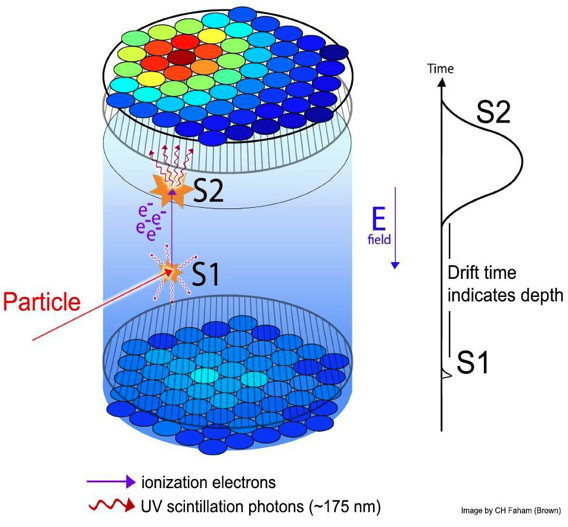
\includegraphics[width=0.7\textwidth]{Principle3.png}
    \caption{Working principle of a DM detector \cite{Akerib:2015gmi}.}
    \label{fig:working}
\end{figure}

With this process, the cross section of the interactions of WIMPs and the molecules of the TPC can be determined. So far, only upper limits of the cross section are found in several experiments (see figure \ref{fig:Sens}). The shape of the curves are like this due to two aspects. For low masses the energy of the WIMP is not high enough to be detected. So less interactions will take place in the detectors and the sensitivity becomes more worse. For high WIMP masses the interaction rate is also lower because $R\propto m_\chi^{-1}$ (see eq. (\ref{interaction_rate})).
Some of the existing experiments are covered in section \ref{sec:current_exp}.
\subsubsection{Content TPC}
One can chose the material inside the TPC. Mostly liquid noble-gasses are used. Xenon is the most used noble-gas, although also argon is being used. The advantage of using xenon is that it is sensitive to both spin-dependent and spin-independent interactions \cite{Aprile:2013doa}, it is self-shielding due to a high density (so more xenon can be used for measuring) \cite{Undagoitia:2015gya} and it is stable.


% (Afbeelding 1 van \href{https://www.symmetrymagazine.org/image/april-2012-dark-matter-underground}{Symmetry magazine}, afbeelding 2 van \href{https://phys.org/news/2017-03-dark-ton.html}{Phys.org})


\subsection{Current experiments}
\label{sec:current_exp}
At the moment, several experiments on the direct detection of dark matter are being done. Some of them are discussed here: the PandaX-II detector in Sichuan, China, the LUX detector in South Dakota, USA and the XENON1T detector in Abruzzo, Italy.

\subsubsection{PandaX-II}
\label{sec:PandaX}\textcolor{red}{P}article \textcolor{red}{and A}strophysical \textcolor{red}{X}enon Detector II (PandaX-II) is a dark matter experiment situated in the region Sichuan in the People's Republic of China. It is a detector with 300 kg of effective liquid xenon target \cite{Liu2015} (more details and latest results in e.g. \cite{Cui:2017nnn}).\\

\begin{figure}[h]
    \centering
    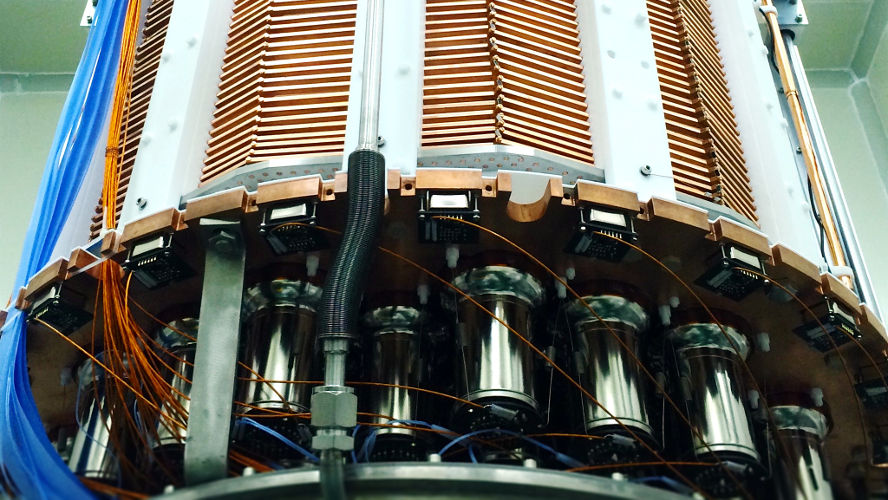
\includegraphics[width=0.9\textwidth]{pandax.jpg}
    \caption{PandaX detector \cite{SJTU}.}
    \label{fig:PandaX}
\end{figure}

\subsubsection{LUX}
\label{sec:LUX}The \textcolor{red}{L}arge \textcolor{red}{U}nderground \textcolor{red}{X}enon experiment (LUX) in the Sanford Underground Research Facility near Lead, South Dakota, USA is an 30 million US dollar costing experiment looking for dark matter at 1,480 meters depth \cite{Reich2013}. The latest results are written in \cite{Akerib:2016vxi}. For more details see e.g. \cite{Akerib:2012ys}.

%LUX (Afbeelding van \href{https://physicsworld.com/a/dark-matter-constraints-tightened-after-lux-no-shows/}{Physics World})\\

\begin{figure}[h]
    \centering
    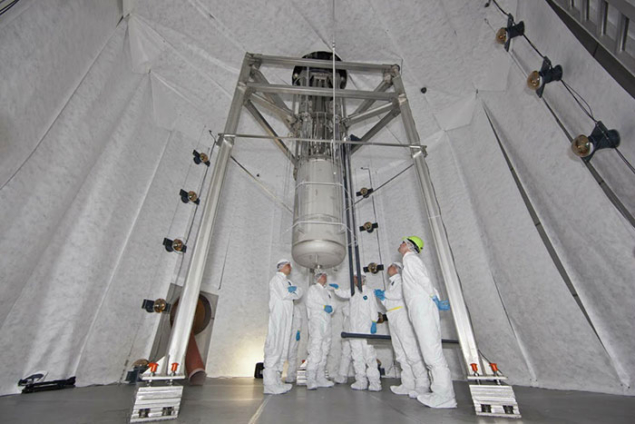
\includegraphics[width=0.9\textwidth]{lux.jpg}
    \caption{LUX detector \cite{PhysWorld}.}
    \label{fig:LUX}
\end{figure}

\subsubsection{XENON1T}
\label{sec:XENON}In the Gran Sasso d'Italia - a mountain massive in Southern Italy - several scientific experiments are being done. One of them is the XENON1T dark matter detector. 1.3 tonne of liquid xenon is used to take the latest data \cite{Aprile:2018dbl}. Currently, it is the most sensitive dark matter detector (see figure \ref{fig:Sens}). It set the upper limit for the WIMP-nucleon spin-independent cross section for WIMPs with mass $m_\chi =30\ GeV/c^2$ at $\sigma_\chi^{m=30\ GeV/c^2}<4.1\times 10^{-47}\ cm^2$.
%(Afbeelding van \href{http://www.physics.purdue.edu/darkmatters/xenon1t/?tag=xenon1t}{Perdue University})

\begin{figure}[h]
    \centering
    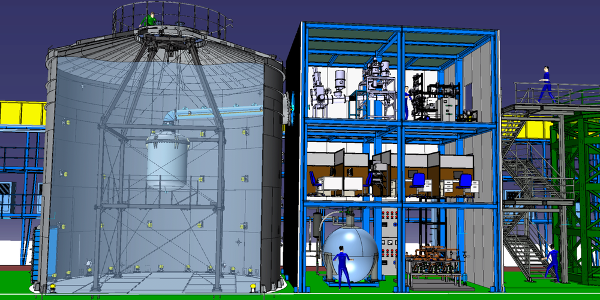
\includegraphics[width=0.9\textwidth]{Xenon1T.png}
    \caption{XENON1T detector \cite{Perdue}.}
    \label{fig:XENON1T}
\end{figure}

\subsubsection{DarkSide}
\label{sec:DarkSide}Next to the XENON1T experiment the DarkSide experiment is running in the Gran Sasso National Laboratory. This is a direct dark matter detector with TPCs based on argon \cite{Agnes:2015ftt, Agnes:2018mon, Edkins:2017qct}. This detector is a few orders of magnitude less sensitive than the detectors with xenon-based TPCs (see figure \ref{fig:Sens}).

\subsubsection{SuperCDMS}
\label{sec:SuperCDMS}In the Soudan Underground Mine, Minnesota, a dark matter detector named SuperCDMS (\textcolor{red}{Super} \textcolor{red}{C}ryogenic \textcolor{red}{D}ark \textcolor{red}{M}atter \textcolor{red}{S}earch) is build (see figure \ref{fig:SuperCDMS}). This detector works with silicon crystal cooled down to $33\ mK$ to measure phonons (heat) \cite{Agnese:2018col}. More on SuperCDMS in \cite{Agnese:2013jaa, Agnese:2014aze, Agnese:2015nto}.

\begin{figure}
    \centering
    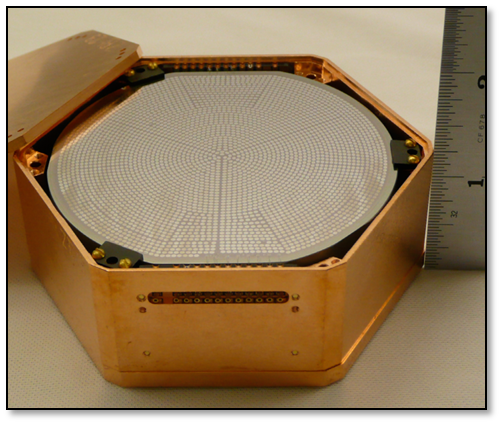
\includegraphics[width=.9\textwidth]{SuperCDMS.png}
    \caption{One of the modules used in the SuperCDMS detector \cite{SuperCDMSphoto}.}
    \label{fig:SuperCDMS}
\end{figure}

\subsubsection{CRESST-II}
\label{sec:CRESST} The \textcolor{red}{C}ryogenic \textcolor{red}{R}are \textcolor{red}{E}vent \textcolor{red}{S}earch with \textcolor{red}{S}uperconducting \textcolor{red}{T}hermometers-II is detecting dark matter with photons and phonons \cite{Angloher:2015ewa}. In this experiment a $CaWO_4$ crystal is used. Most of the energy deposition is in the form of heat. Less than $5\%$ of the energy goes into the scintillation. For more information on CRESST, see \cite{Bravin:1999fc,Angloher:2014myn,Petricca:2017zdp}.

\begin{figure}
    \centering
    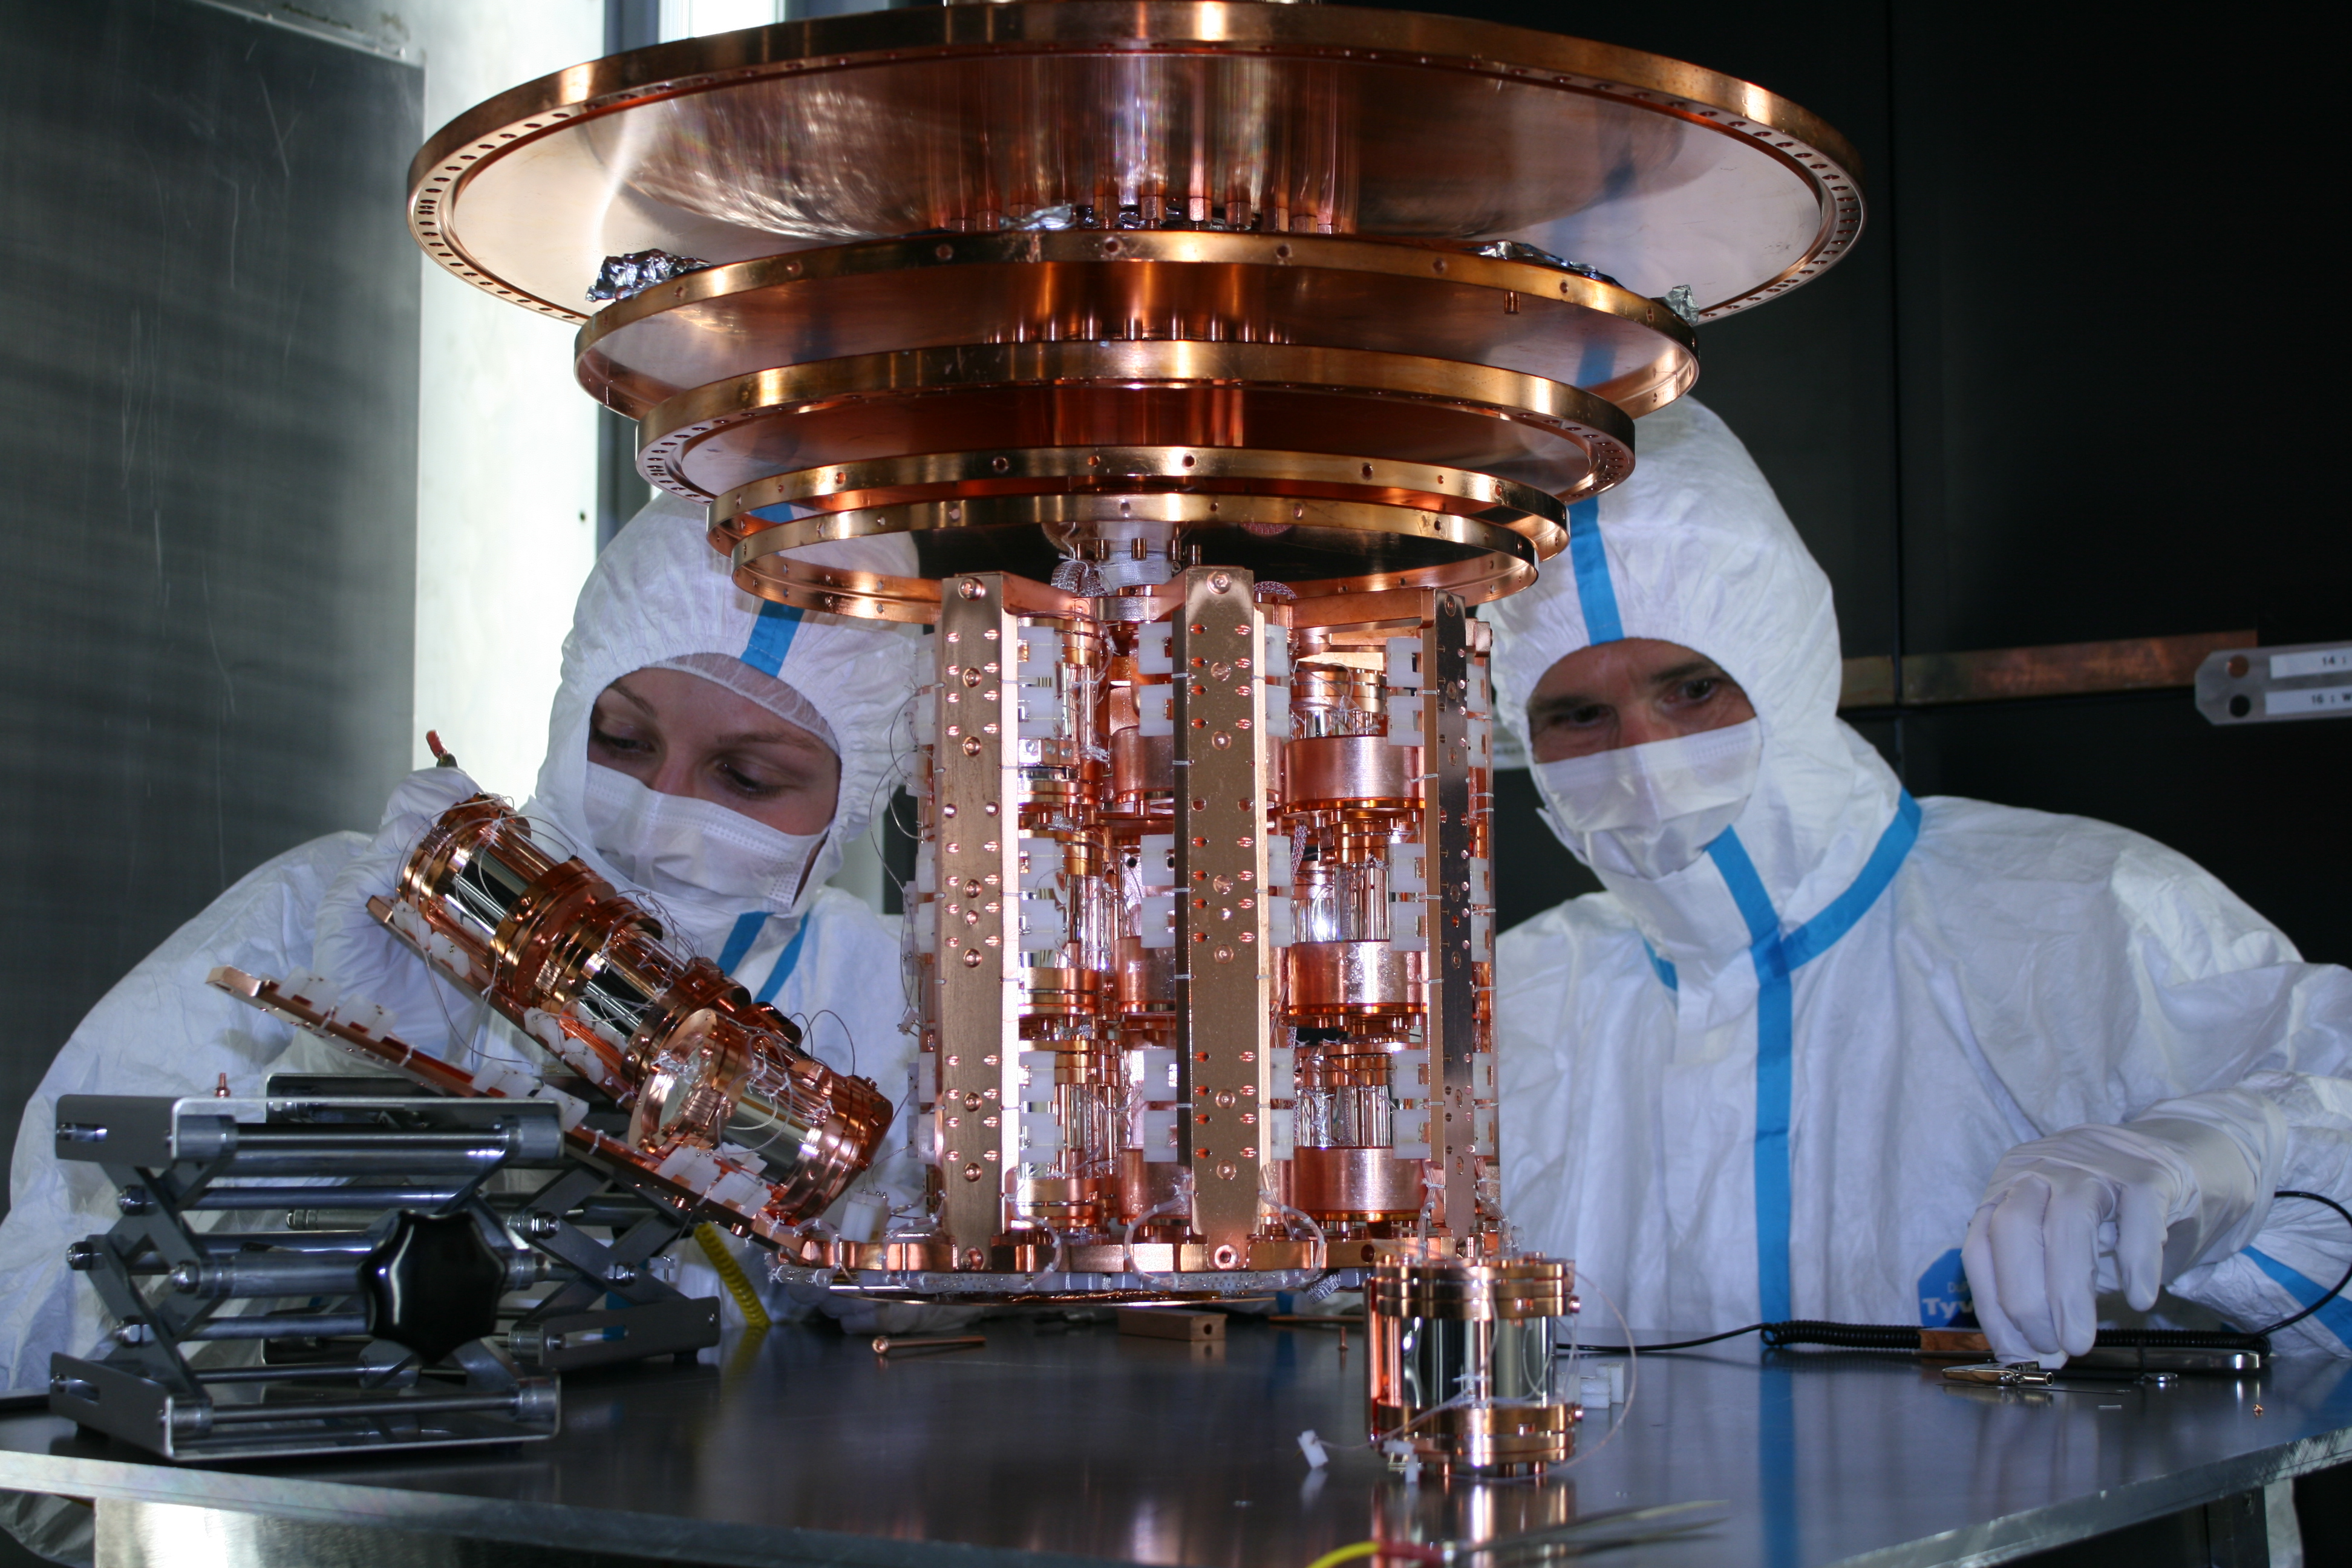
\includegraphics[width=0.9\textwidth]{CRESST.jpg}
    \caption{Installation of CRESST \cite{CRESSTphoto}.}
    \label{fig:CRESST}
\end{figure}

\begin{figure}[h]
    \centering
    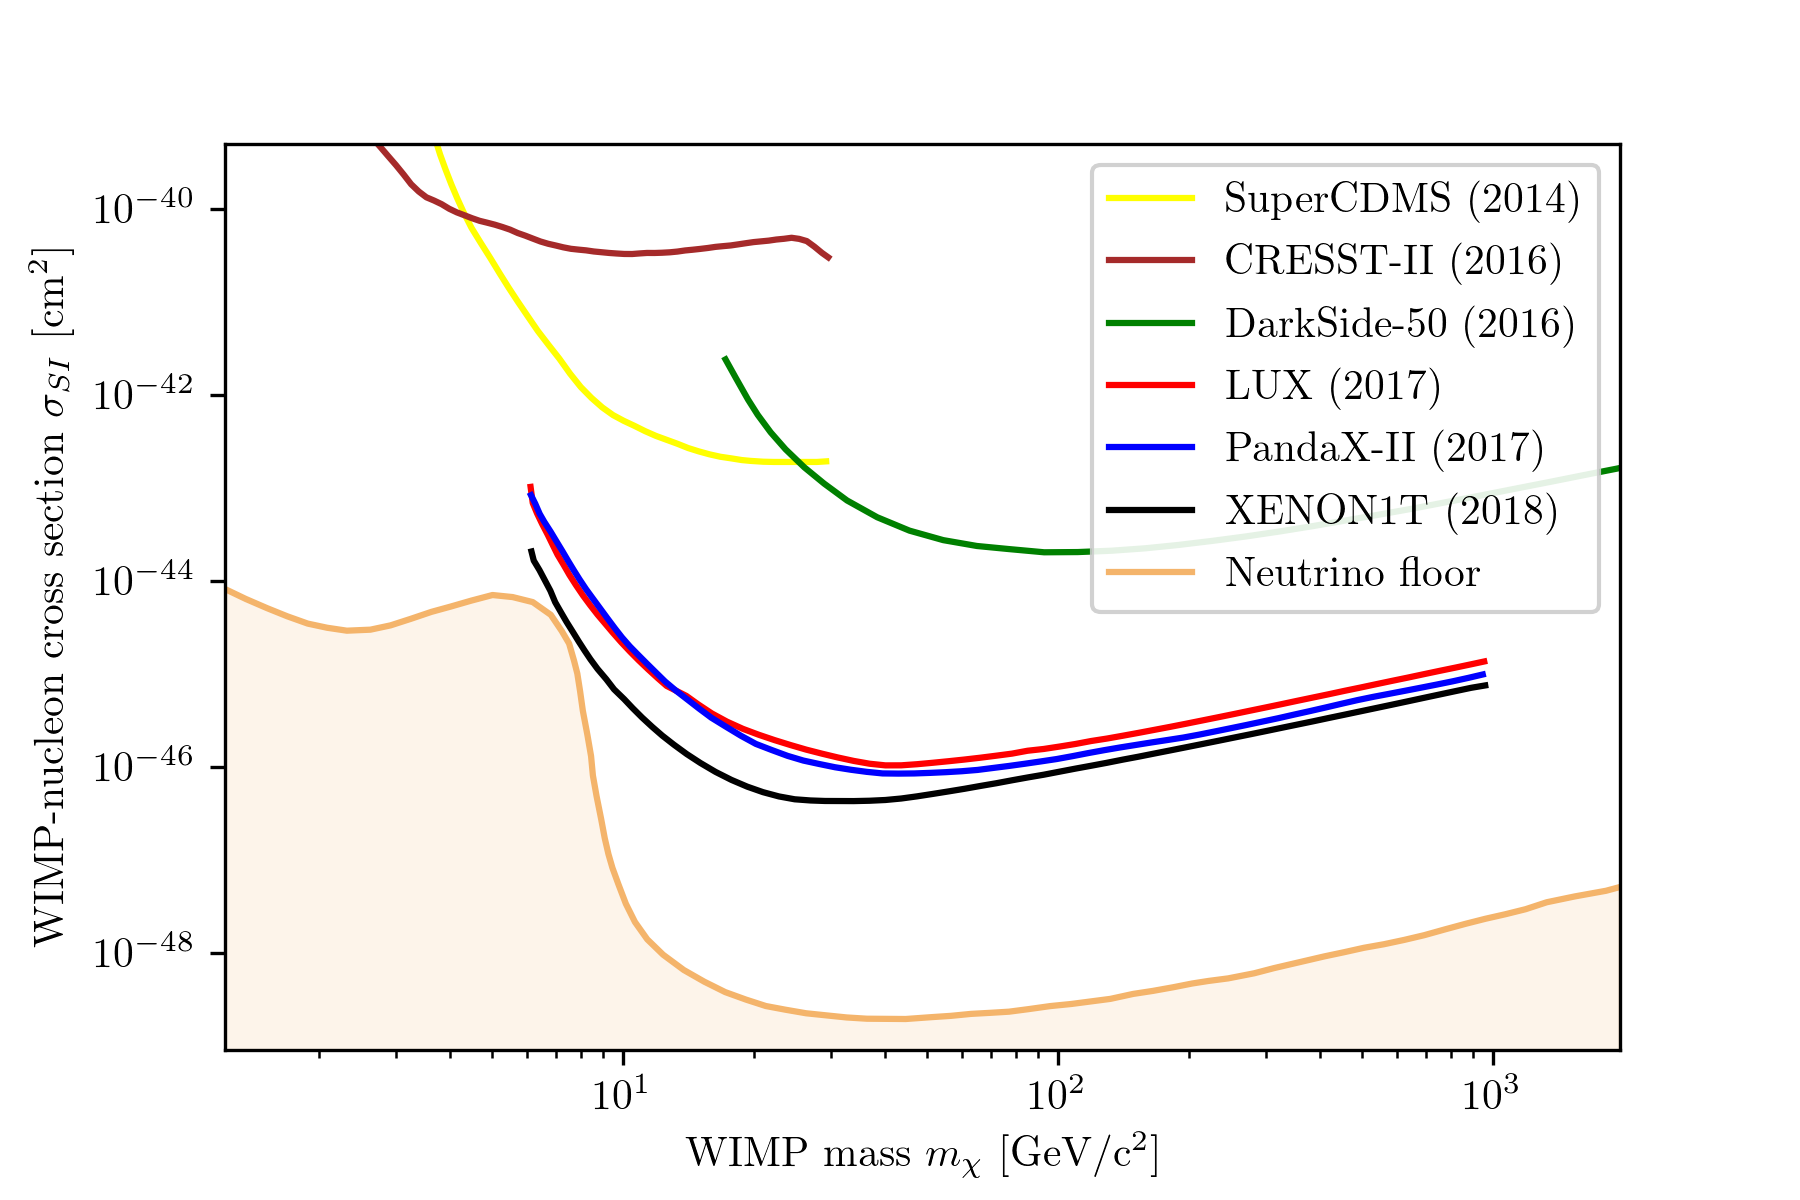
\includegraphics[width=0.7\textwidth]{Sens_plot_floor.png}
    \caption{Sensitivity plot. Data from SuperCDMS \cite{Agnese:2014aze}, CRESST-II \cite{Angloher:2015ewa}, DarkSide \cite{Agnes:2015ftt}, PandaX \cite{Cui:2017nnn}, LUX \cite{Akerib:2016vxi}, XENON1T \cite{Aprile:2018dbl} and floor \cite{Liu:2017drf}.}
    \label{fig:Sens}
\end{figure}

\subsection{Future experiments}
In the search for dark matter particles one tries to bring down the sensitivity curves (as in figure \ref{fig:Sens}). This is being done with upgrades of existing experiments and building new detectors. Some of them are discussed in this section.

\subsubsection{XENONnT}
The XENON collaboration is working on XENONnT as upgrade of the XENON1T experiment. It is going to be a 5.9 tonne sister of the XENON1T detector \cite{Aprile:2018dbl}. The planning is to be running in 2019 \cite{APPEC}.
%XENONnT ready 2019 (https://science.purdue.edu/xenon1t/)

%\subsubsection{PandaX-30T}
%PandaX-30T

\subsubsection{DARWIN}
DARWIN is a new to build dark matter detector. DARWIN stands for \textcolor{red}{Dar}k matter \textcolor{red}{WI}MP search with \textcolor{red}{N}obble liquids. It will mainly search for WIMPS until the neutrino floor is reached (for the neutrino floor, see section \ref{sec:floor}) \cite{Aalbers:2016jon}. Also research on axions, the low-energy solar neutrinos and galactic supernovae will be preformed.
%DARWIN (https://arxiv.org/abs/1606.07001)

\subsubsection{LZ}
LZ is a combination of \textcolor{red}{L}UX and \textcolor{red}{Z}EPLIN (\textcolor{red}{Z}on\textcolor{red}{e}d \textcolor{red}{p}roportional scintillation in \textcolor{red}{li}quid \textcolor{red}{n}oble gases). It's currently being built in the Sanford Underground Research Facility. See for more (technical) information \cite{Akerib:2015cja,Mount:2017qzi}.

\subsection{Electron excitation}
\subsubsection{Noble liquids}
\subsubsection{Semiconductors}

 

\FloatBarrier
\section{Neutrino floor \small{\textit{Peter Bosch}}}
\label{sec:floor}
In dark matter direct detection experiments, one always tries to bring down the sensitivity of interaction in the detector. At a certain moment interactions of neutrinos can not longer be neglected. Although neutrinos have a very small cross section, they do interact. So one will measure the neutrinos in the detector. This is called the neutrino floor. In figure \ref{fig:Sens} the neutrino floor is given. The yellow solid line is the place where one interaction has taken place. So beneath this line, interactions with neutrinos can become a problem. In this section we will go into the neutrino floor and how to go beneath it.

\subsection{Origin of neutrinos \small{\textit{Peter Bosch}}}
As said before neutrinos are interacting inside the detectors. These neutrinos are coming from several sources. The main sources are
\begin{enumerate}
    \item the Sun,
    \item the Earth,
    \item the atmosphere,
    \item supernovae and
    \item nuclear reactors.
\end{enumerate}
The neutrino fluxes for these source are given in table \ref{tab:neutrino_flux}.
\begin{table}[]
    \centering
    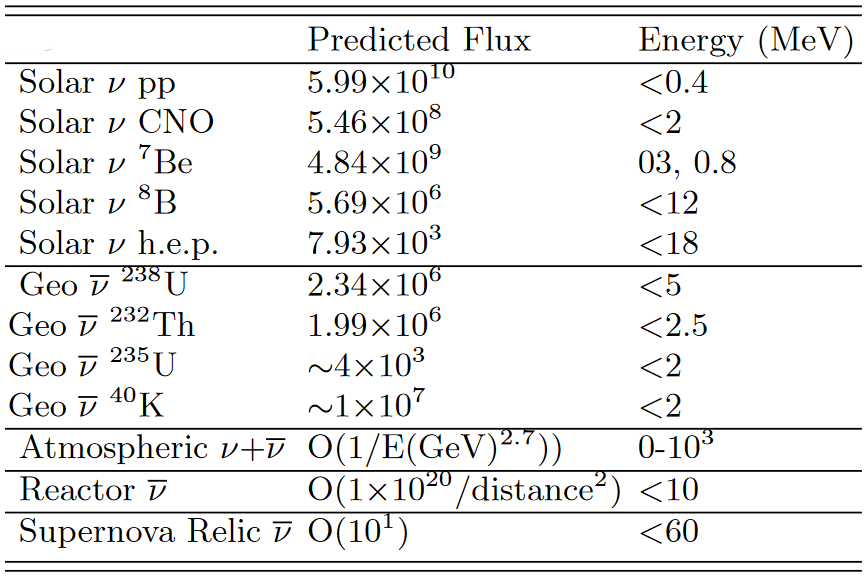
\includegraphics[width=.8\textwidth]{Neutrino_fluxes.PNG}
    \caption{Neutrino fluxes in $cm^{-2}\ s^{-1}$, the energy range and their sources \cite{Monroe:2007xp}.}
    \label{tab:neutrino_flux}
\end{table}
\subsubsection{Solar neutrinos}
In the core of the Sun lots of nuclear fusion reactions happen. The main reaction cycle of the Sun is the proton cycle, but also other cycles as the CNO cycle provides the Sun energy \cite{Bonventre:2018hyd}. With some of these reactions neutrinos are created. For example, in the full proton-proton cycle,
\begin{align}
    {}^1\text{H}+{}^1\text{H}&\rightarrow {}^2\text{H}+e^++\nu_e \nonumber\\
    {}^2\text{H} + {}^1\text{H} &\rightarrow ^3\text{He}+\gamma \nonumber\\
    2\ {}^3\text{He} &\rightarrow {}^4\text{He}+2\ {}^1\text{H},
\end{align}
two neutrinos are created. These neutrinos will travel from the core to the outer shell of the Sun without having any reaction (or at least very little). From there they travel through space. Some of the neutrinos - $2\pi R_\oplus^2 / 4\pi d^2 \approx 10^{-7}\%$ - are going towards Earth. They can also go through the Earth atmosphere without a negligible amount of interactions. Again a small fraction of the remaining neutrinos are hitting the detector in the experiments searching for dark matter. Here the neutrinos interact more because the detectors are made very sensitive for this kind of interactions as they are similar for dark matter interactions.

\subsubsection{Atmospheric neutrinos}
In the universe particles are created (e.g. pions). These particles move through space without interacting and are called cosmic rays. In the outer atmosphere pions start to decay creating neutrinos \cite{Fukuda:1998mi,Gaisser:2016obt}. This is dominated by the decays
\begin{equation}
    \pi^+\rightarrow\mu^++\nu_\mu
\end{equation}
and
\begin{align}
    \mu^+\rightarrow e^++\bar{\nu}_\mu+\nu_e.
\end{align}
As before with solar neutrinos, they don't interact in the remaining atmosphere. The non-neutrino particles will further decay and create neutrinos. All these neutrinos can interact in a dark matter detector.

\subsubsection{Supernovae neutrinos}
At the end of their lifetime, starts explodes \cite{raffelt1996stars}. These explosions are called supernovae. Some supernovae create neutrinos \cite{Beacom:2010kk}. The first neutrinos were detected in 1987 with Kamiokande \cite{Totsuka:1988iyh}. The neutrinos were coming from a supernova called SN1987A in the Large Magellanic Cloud.

\subsubsection{Other neutrinos}
As stated before and can be seen in table \ref{tab:neutrino_flux} there are, besides solar, atmospheric and supernovae neutrinos, two other sources of neutrinos. Some are coming from natural decays in the inner Earth (mostly ${}^{238}U$ and ${}^{232}Th$). Also some neutrinos are created by man-made decays in nuclear reactors.

\subsection{A fundamental limit \small{\textit{Max Briel}}}

It is expected that the neutrino floor will be reached in the coming years; rather sooner than later. This rises the question whether the neutrino background could limit the possible detection of dark matter, because the signal from an neutrino particle looks exactly the same as that of a WIMP in current detectors \cite{Gutlein:2010tq,Billard:2013qya}. Due to their extremely small interaction cross section, neutrinos cannot be shielded from the detector. Thus, they impose a limit on the minimum measurable cross section. This is not a final limit; by increasing the exposure, which depends on the mass and measurement time, it is possible to increase the discovery reach. As shown in figure \ref{discovery_limit}, initially, this scales as $1/MT$, when neutrino interactions are minimum. However, at higher exposures the neutrinos become more important and the discovery limit starts to scale as $1/\sqrt{MT}$. The point where it changes is WIMP mass dependent and is often what is called the neutrino floor. In reality it is still possible to continue the exposure and continue the search below this neutrino limit, therefore, it is a "soft" limit. If the exposure is increased even more, eventually the discovery reach will almost flatten out. This plateau is also known as the "hard" floor, but to reach it the exposure has to be unrealistically high \cite{Wyenberg:2018eyv}. 

The simplest option to surpass this limit is to distinguish nuclear recoil and electron recoil events. 


\begin{figure}[h]
    \centering
    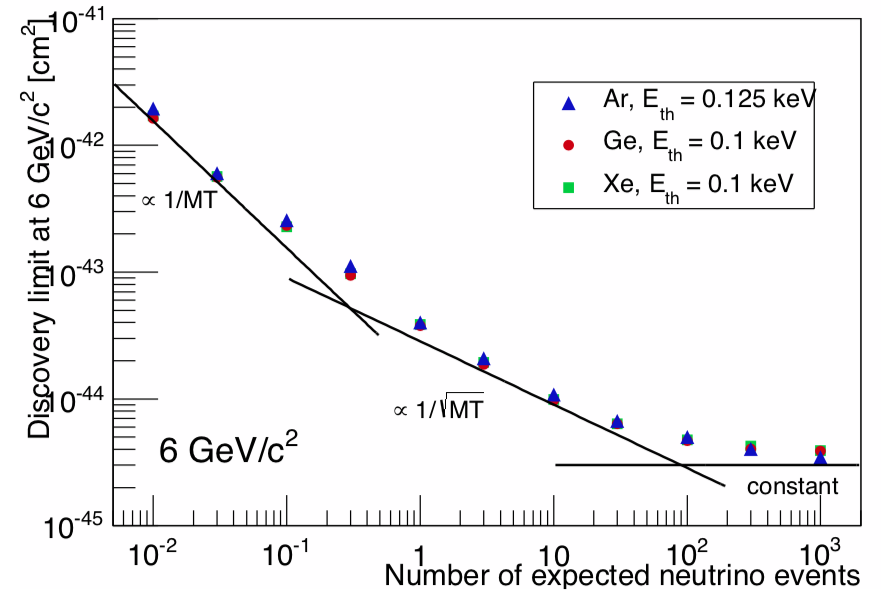
\includegraphics[width=0.9\textwidth]{Discovery_limit.png}
    \caption{Discovery limit vs exposure for a 6 GeV/$c^2$ WIMP with Ge, Xe, Ar for 100 neutrino events in 240, 130, and 430 kg-years. Image from \cite{Billard:2013qya}.}
    \label{discovery_limit}
\end{figure}



\subsection{Continue searching? \small{\textit{Jelle van Urk}}}
\textbf{Jelle}
Direct detection experiments are improving in size and sensitivity for the past couple of years. This means that in the nearby future we will probably reach the neutrino floor, explained in the previous section. This will make the detection for WIMPs even harder, because the scattering interaction events of neutrinos in the detector can be equivalent to a WIMP interaction. Therefore  it's important to understand if it's possible to distinguish the neutrino background events from the dark matter particles. One important step is to better understand the theoretical estimation of the neutrino fluxes. As well as a better measurement to distinguish the different neutrinos entering the detector. 

\subsubsection{Directional experiments}
As described before, most neutrinos are incident from the Sun \cite{Billard:2013qya}. This gives a good opportunity to distinguish them from WIMPs, as the directional signal for these neutrinos would probably be completely different. New experiments are being developed which enable the possibility to measure the incoming direction of WIMPs \cite{Ahlen:2009ev}. 

\subsubsection{Annual modulation}
The DAMA/NaI and DAMA/LIBRA experiments were the first experiment that claimed to have found dark matter \cite{Freese:2012xd}. These results showed an annual modulation of the interaction events which was the highest in June (see figure ...).
\begin{figure}[h]
    \centering
    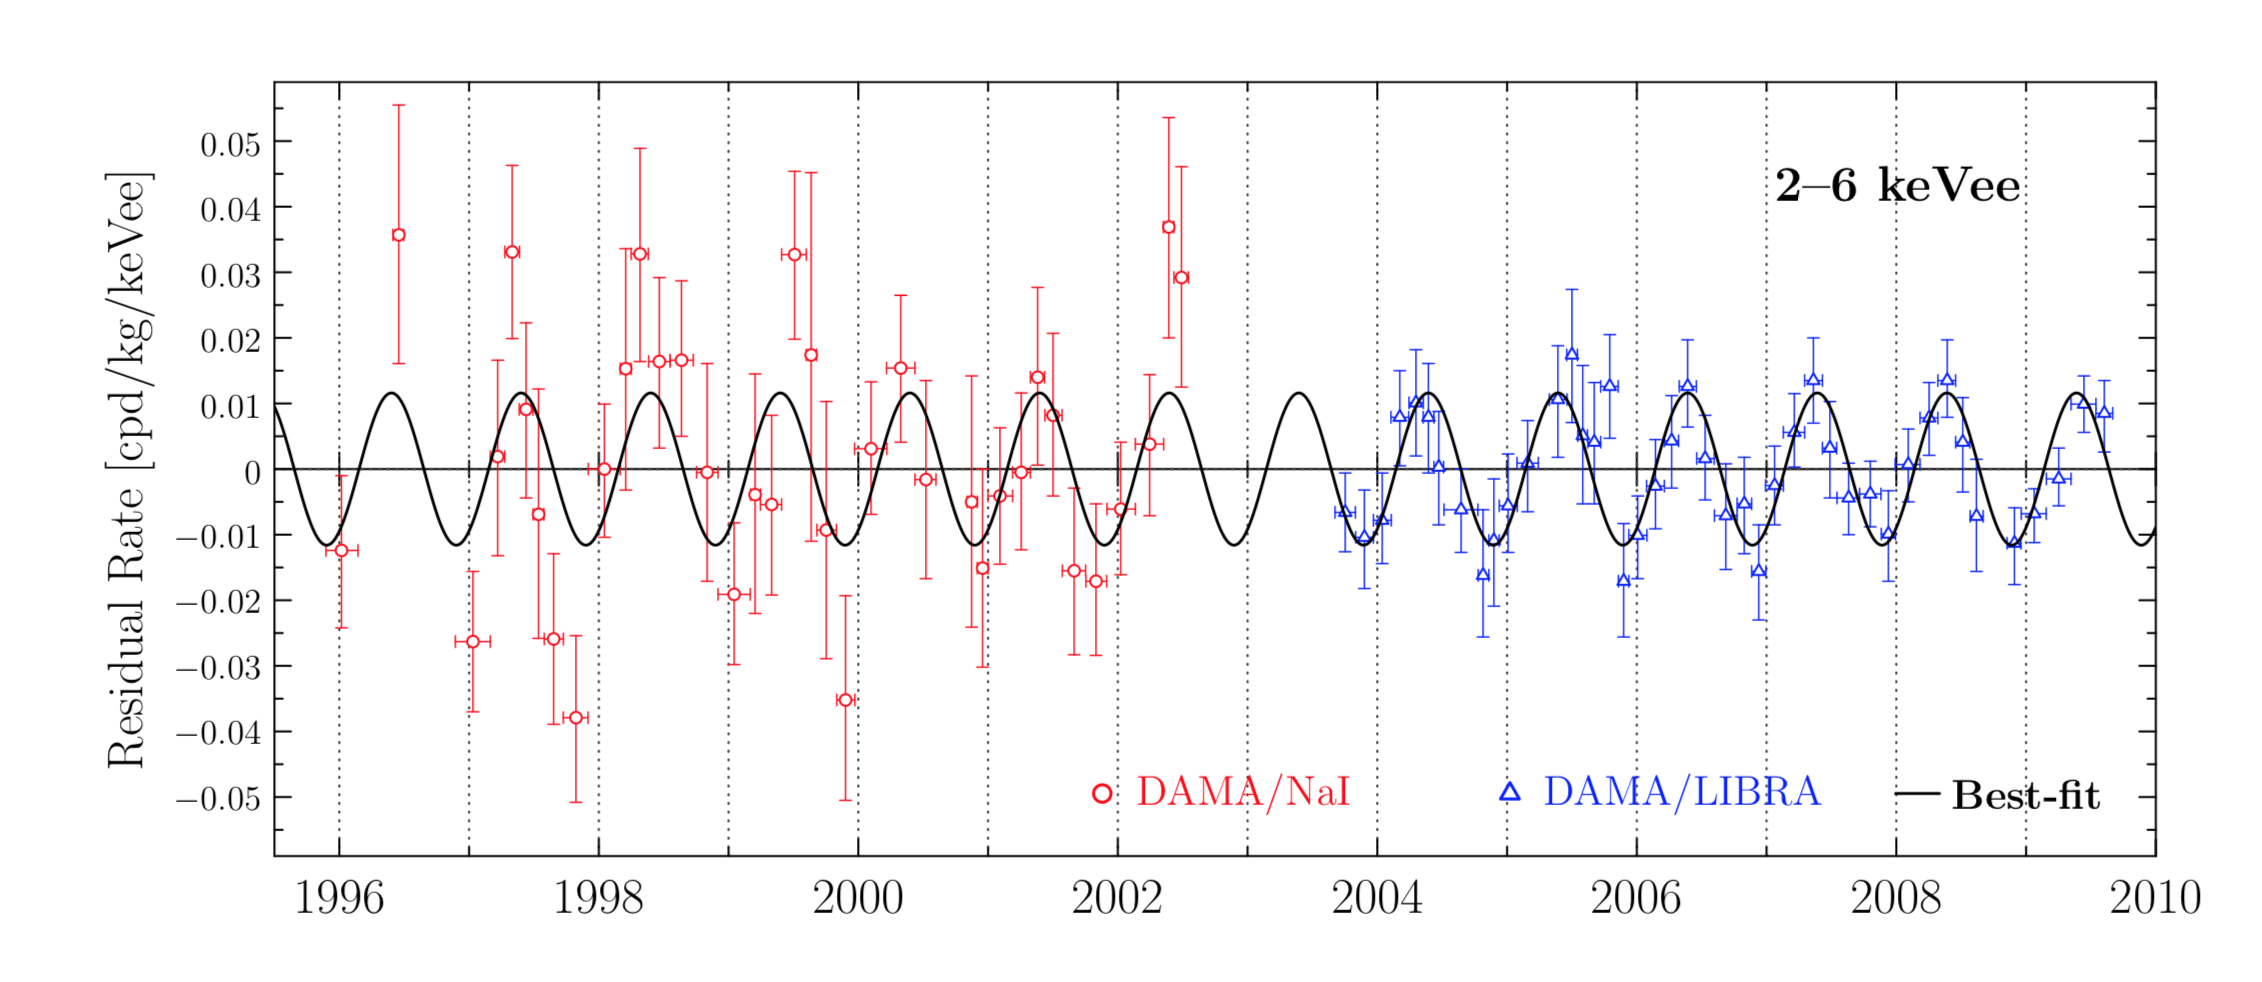
\includegraphics[width=\textwidth]{Annualmodulation.png}
    \caption{}
\end{figure}

\FloatBarrier
\subsubsection{Extraction of neutrino background}
Besides different incoming directions and annual modulation of WIMPs and neutrinos, there will always be some neutrino scattering events which will be similar to those of WIMPs. Therefore it is useful to investigate the how a neutrino only distribution would look like, thus a reconstruction of the neutrino background. 

In the left graph of figure ... you can see a simulated distribution of neutrinos in the range where they could mimic the WIMPs. This simulation is done with Xenon as target nucleus. The legend shows the different origin of neutrinos. The left top of the figure, low mass with high cross section, consist mostly of neutrinos that are incident from the Sun. This is different for atmospheric and diffuse supernova neutrino background (DSNB), which have a higher mass and lower energy (bottom right).
The right graph of this figure shows a accumulation of all the different neutrinos. However, this time a simulation is done with different target nuclei: Xenon, Germanium, Argon, Silicon, Neon and Fluorine. Again, it's obvious that the solar neutrinos (low mass, high cross section) are the most abundant. Xenon and Germanium, which are heaviest of the target nuclei, also show a non-negligible amount of events for atmospheric and SN neutrinos. 
These two graphs show some valuable simulated data. The different target nuclei give slightly different signals. Hence, these target nuclei could be used to distinguish the neutrino background from the WIMPs.
\begin{figure}[h]
    \centering
    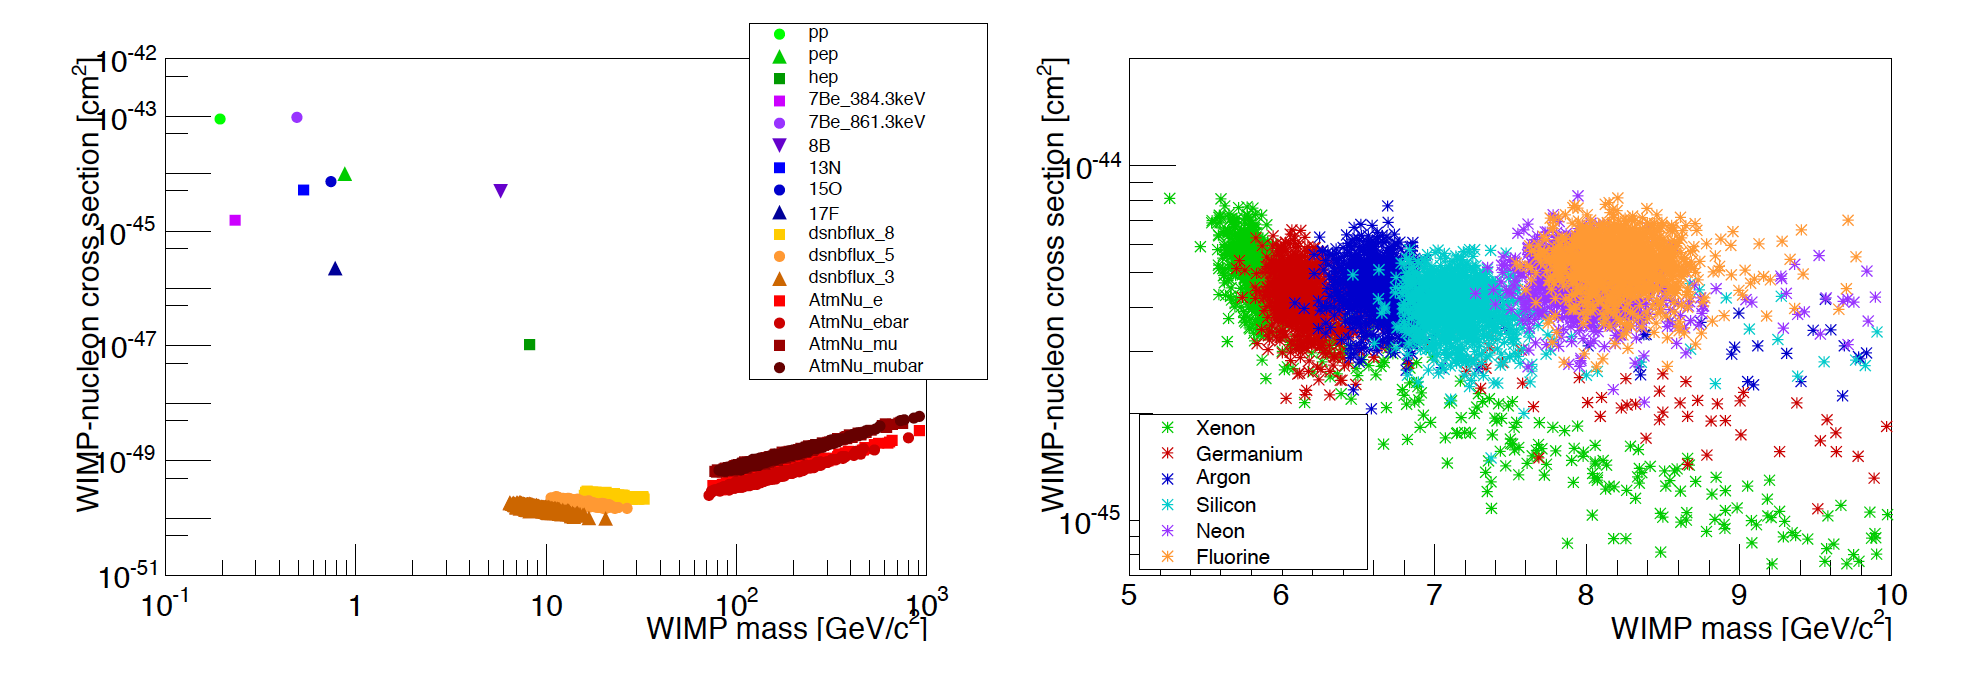
\includegraphics[width=\textwidth]{Neutrinos3.png}
    \caption{\cite{Billard:2013qya}}
\end{figure}







% =============================================================
\FloatBarrier

\
\newpage
\bibliographystyle{unsrt}
\bibliography{refs}

\end{document}

%About nuclear form factor
%http://personalpages.manchester.ac.uk/staff/Sean.Freeman/pc3121/formfactors.pdf

%Reconstruction
%https://arxiv.org/pdf/astro-ph/0703651.pdf